%%%%%%%%%%%%%%%%%%%%%%%%%%%%%%%%%%%%%%%%%%%%%%%%%%%%%%%%%%
%%%%%%%%%%%%%%%%%%%%%%%%%%%%%%%%%%%%%%%%%%%%%%%%%%%%%%%%%%
%%%%%%%%%%%%%%%%%%%%%%%%%%%%%%%%%%%%%%%%%%%%%%%%%%%%%%%%%%
%%%%%%%%%%%%%%%%%%%%%%%%%%%%%%%%%%%%%%%%%%%%%%%%%%%%%%%%%%
\chapter{Mixing}

%%%%%%%%%%%%%%%%%%%%%%%%%%%%%%%%%%%%%%%%%%%%%%%%%%%%%%%%%%
%%%%%%%%%%%%%%%%%%%%%%%%%%%%%%%%%%%%%%%%%%%%%%%%%%%%%%%%%%
%%%%%%%%%%%%%%%%%%%%%%%%%%%%%%%%%%%%%%%%%%%%%%%%%%%%%%%%%%
\section{Physics}

We consider the resolution of the 2D Navier-Stokes equations coupled to a passive scalar convection-diffusion equation in a cavity of length $L$ and height $H$ with moving boundary conditions on all sides. The resulting system is driven by the following set of equations:

\begin{equation}
\label{eq:mixing}
\begin{split}
	\nabla \cdot \V{u} 						&= 0, \\
	\partial_t \V{u} + (\V{u} \cdot \nabla) \, \V{u} 	&= -\nabla p + \frac{1}{\re} \nabla^2 \V{u}, \\
	\partial_t c + (\V{u} \cdot \nabla) \, c 			&= \frac{1}{\pe} \nabla^2 c,
\end{split}
\end{equation}

where $\V{u}$ and $p$ are respectively the non-dimensional velocity and pressure of the fluid, and $c$ is the concentration of a passive species. The dynamics of the system (\ref{eq:mixing}) are controlled by two adimensional numbers. First, the Reynolds number $\re$, which represents the ratio between inertial and viscous forces:

\begin{equation*}
	\re = \frac{U L}{\nu},
\end{equation*}

where $U$ and $L$ are respectively the reference velocity and length values, and $\nu$ is the kinematic viscosity of the fluid. Second, the P\'eclet number $\pe$, which represents the ratio between the advective and diffusive transport rates:

\begin{equation*}
	\pe = \frac{U L}{D},
\end{equation*}

where $D$ is the diffusion coefficient of the considered species. In essence, a system with a high $\pe$ value presents a negligible diffusion, and scalar quantities move primarily due to fluid convection. The system (\ref{eq:mixing}) is completed by the following initial and boundary conditions:

\begin{equation}
\label{eq:mixing_bc}
\begin{split}
	\V{u}(x,y,0)	= 0 &\text{ and } c(x,y,0)	= c_0 \mathbb{1}_{\substack{ {x_\text{min} \leq x \leq x_\text{max}}\\ {y_\text{min} \leq y \leq y_\text{max}} }} \\
	\V{u}(x=0,y,t)	= (0, v_l) &\text{ and } \V{u}(x=L,y,t) = (0, v_r), \\
	\V{u}(x,y=0,t)	= (u_b, 0) &\text{ and } \V{u}(x,y=H,t) = (u_t, 0), \\
	\partial_y c(x,y=0,t) 	= 0 &\text{ and } \partial_y c(x,y=H,t) = 0, \\
	\partial_x c(x=0,y,t) = 0 &\text{ and } \partial_x c(x=L,y,t) = 0,
\end{split}
\end{equation}

where $\mathbb{1}$ is the indicator function, and $v_l$, $v_r$, $u_b$ and $u_t$ are user-defined values. In essence, the boundary conditions (\ref{eq:mixing_bc}) correspond to a multiple lid-driven cavity, where tangential velocity can be imposed independently on all sides, with an initial patch of concentration in the center of the domain.  Snapshots of the evolution of the system in time with $(v_l, v_r, u_b, u_t) = (0, 0, 1.0, -1.0)$ are presented in figure \ref{fig:mixing_example}.

%%%%%%%%%%%%
%%%%%%%%%%%%
\begin{figure}
\centering
%%%%%%%%%%%%
\pgfdeclarelayer{background}
\pgfsetlayers{background,main}
%%%%%%%%%%%%
%%%%%%%%%%%%

\begin{subfigure}[t]{.22\textwidth}
	\centering
	\fbox{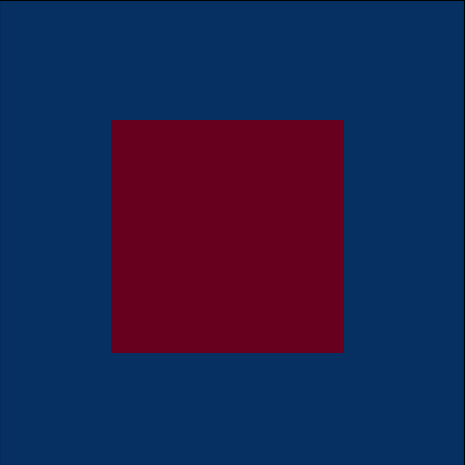
\includegraphics[width=\textwidth]{fig/mixing/example_t0.png}}
    	\caption{$t=0$}
	\label{fig:mixing_example_0}
\end{subfigure} \quad
\begin{subfigure}[t]{.22\textwidth}
	\centering
	\fbox{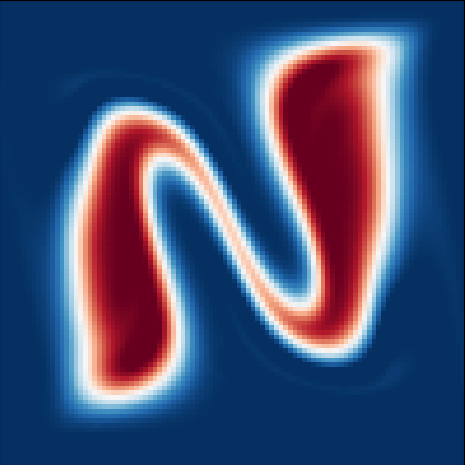
\includegraphics[width=\textwidth]{fig/mixing/example_t10.png}}
    	\caption{$t=10$}
	\label{fig:mixing_example_10}
\end{subfigure} \quad
\begin{subfigure}[t]{.22\textwidth}
	\centering
	\fbox{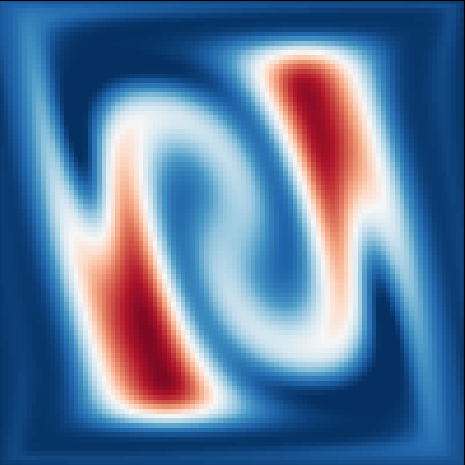
\includegraphics[width=\textwidth]{fig/mixing/example_t30.png}}
    	\caption{$t=30$}
	\label{fig:mixing_example_30}
\end{subfigure} \quad
\begin{subfigure}[t]{.22\textwidth}
	\centering
	\fbox{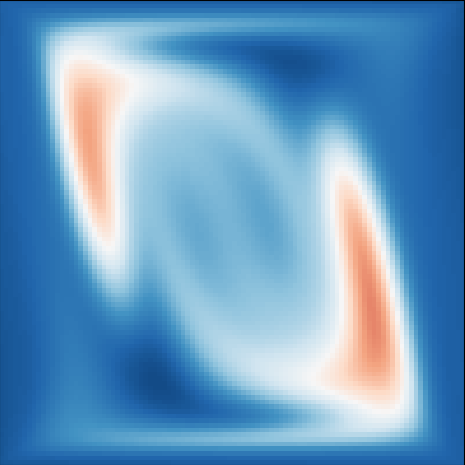
\includegraphics[width=\textwidth]{fig/mixing/example_t60.png}}
    	\caption{$t=60$}
	\label{fig:mixing_example_60}
\end{subfigure}

%%%%%%%%%%%%
\caption{\textbf{Evolution of the concentration in time} with constant boundary conditions $(v_l, v_r, u_b, u_t) = (0, 0, 1.0, -1.0)$.}
\label{fig:mixing_example}
\end{figure} 
%%%%%%%%%%%%
%%%%%%%%%%%%

%%%%%%%%%%%%%%%%%%%%%%%%%%%%%%%%%%%%%%%%%%%%%%%%%%%%%%%%%%
%%%%%%%%%%%%%%%%%%%%%%%%%%%%%%%%%%%%%%%%%%%%%%%%%%%%%%%%%%
%%%%%%%%%%%%%%%%%%%%%%%%%%%%%%%%%%%%%%%%%%%%%%%%%%%%%%%%%%
\section{Discretization}

The system (\ref{eq:mixing}) is discretized using a structured finite volume incremental projection scheme with centered fluxes. For simplicity, the scheme is solved in a fully explicit way, except for the resolution of the Poisson equation for pressure. As is standard, a staggered grid is used for the finite volume scheme: the horizontal velocity is located on the west face of the cells, the vertical velocity is on the south face of the cells, while the pressure and temperature are located at the center of the cells.

%%%%%%%%%%%%%%%%%%%%%%%%%%%%%%%%%%%%%%%%%%%%%%%%%%%%%%%%%%
%%%%%%%%%%%%%%%%%%%%%%%%%%%%%%%%%%%%%%%%%%%%%%%%%%%%%%%%%%
%%%%%%%%%%%%%%%%%%%%%%%%%%%%%%%%%%%%%%%%%%%%%%%%%%%%%%%%%%
\section{Environment}

In the following, we set $H=1$, $L=1$, $\Delta X = x_\text{max} - x_\text{min} = 0.5$, $\Delta Y = y_\text{max} - y_\text{min} = 0.5$, and $c_0 = 1$. The control is performed by letting the agent adjust the tangential velocities at the boundaries of the domain. We use a discrete action space of dimension $4$, with the following actions:

\begin{equation}
\label{eq:mixing_actions}
\begin{split}
	a = 0 &\iff (v_l, v_r, u_b, u_t) = (0, 0, u_\text{max}, -u_\text{max}) \\
	a = 1 &\iff (v_l, v_r, u_b, u_t) = (0, 0, -u_\text{max}, u_\text{max}) \\
	a = 2 &\iff (v_l, v_r, u_b, u_t) = (-u_\text{max}, u_\text{max}, 0, 0) \\
	a = 3 &\iff (v_l, v_r, u_b, u_t) = (u_\text{max}, -u_\text{max}, 0, 0),
\end{split}
\end{equation}

where $u_\text{max} = \frac{\re \nu}{L}$. The non-dimensional numbers are chosen as $\re = 100$ and $\pe = \num{1e4}$, which corresponds to a low diffusion species. For simplicity, no temporal interpolation is performed between actions. The spatial discretization step is set as $\Delta x = 0.01$, while the numerical time step is $\Delta t = 0.002$. The action time-step $\Delta t_\text{act}$ is equal to $0.5$ time units, with the total episode length being fixed to $50$ time units, corresponding to $100$ actions. The observations provided to the agent are the temperatures and their derivatives collected on a grid of $n_p \times n_p$ probes evenly spaced in the computational domain. The resulting set of observations is flattened in a vector of size $2 \times (n_h+1)$. The reward at each time-step is simply set as the average absolute distance of the concentration field to a target uniform value: 

\begin{equation}
	r(t) = - \lVert c - c_t \rVert_1 \text{ with } c_t = \frac{\Delta X \Delta Y}{L H} c_0.
\end{equation}

Finally, each episode starts with a null velocity field and an initial square patch of concentration $c_0$ as shown in figure \ref{fig:mixing_example_0}.

%%%%%%%%%%%%%%%%%%%%%%%%%%%%%%%%%%%%%%%%%%%%%%%%%%%%%%%%%%
%%%%%%%%%%%%%%%%%%%%%%%%%%%%%%%%%%%%%%%%%%%%%%%%%%%%%%%%%%
%%%%%%%%%%%%%%%%%%%%%%%%%%%%%%%%%%%%%%%%%%%%%%%%%%%%%%%%%%
\section{Results}

The environment as described in the previous section is referred to as \codeinline{mixing-v0}, and its default parameters are provided in table \ref{table:mixing_parameters}. In this section, we provide some results related to its resolution using a \textsc{ppo} agent (see the general hyperparameters in table \ref{table:default_ppo_parameters}), with the specificity that the entropy bonus parameter is reduced to $\beta = 0.001$. For the training, we set $n_\text{rollout} = 1000$, $n_\text{batch} = 2$, $n_\text{epoch} = 32$ and $n_\text{max} = 600k$.

%The score curve obtained with the PPO algorithm is presented in \ref{fig:rayleigh_score}, while the time evolution of the Nusselt for the controlled versus uncontrolled cases are shown in figure \ref{fig:rayleigh_nusselt}. As can be observed, the agent manages to devise a set of transition actions toward a stationary state with $\nus (t) = 1$. The results of figure \ref{fig:rayleigh_nusselt} are in line with those of \cite{beintema2020}. In figure \ref{fig:rayleigh_fields}, we present the evolution of the temperature field during the first steps of the environment under the control of the agent using the default parameters.

%%%%%%%%%%%
%%%%%%%%%%%
\begin{table}
    \footnotesize
    \caption{\textbf{Default parameters used for the \codeinline{mixing-v0} environment.}}
    \label{table:mixing_parameters}
    \centering
    \begin{tabular}{rll}
        \toprule
        \codeinline{L}			& length of the domain					& $1$\\
	\codeinline{H}			& height of the domain					& $1$\\
	\codeinline{re}			& Reynolds number						& $\num{1e2}$\\
	\codeinline{pe}			& P\'eclet number						& $\num{1e4}$\\
	\codeinline{side}		& initial side length of concentration patch		& $0.5$\\
	\codeinline{c0}			& initial concentration					& $1$\\
        \bottomrule
    \end{tabular}
\end{table}
%%%%%%%%%%%
%%%%%%%%%%%
%
%%%%%%%%%%%%%
%%%%%%%%%%%%
\begin{figure}
\centering
%%%%%%%%%%%%
\begin{tikzpicture}[	trim axis left, trim axis right, font=\scriptsize,
				upper/.style={	name path=upper, smooth, draw=none},
				lower/.style={	name path=lower, smooth, draw=none},]
	\begin{axis}[	xmin=0, xmax=500000, scale=0.75,
				ymin=-6, ymax=0,
				scaled x ticks=false,
				xtick={0, 100000, 200000, 300000, 400000, 500000},
				xticklabels={$0$,$100k$,$200k$,$300k$,$400k$,$500k$},
				legend cell align=left, legend pos=south east,
				legend style={nodes={scale=0.8, transform shape}},
				every tick label/.append style={font=\scriptsize},
				grid=major, xlabel=transitions, ylabel=score]
				
		\legend{no control, \ppo, \ddpg}
		
		\addplot[thick, opacity=0.7, dash pattern=on 2pt]	coordinates {(0,-3.5) (500000,-3.5)};
		
		\addplot [upper, forget plot] 				table[x index=0,y index=7] {fig/burgers/ppo.dat};
		\addplot [lower, forget plot] 				table[x index=0,y index=6] {fig/burgers/ppo.dat}; 
		\addplot [fill=blue3, opacity=0.5, forget plot] 	fill between[of=upper and lower];
		\addplot[draw=blue1, thick, smooth] 			table[x index=0,y index=5] {fig/burgers/ppo.dat}; 
		
		\addplot [upper, forget plot] 				table[x index=0,y index=7] {fig/burgers/ddpg.dat};
		\addplot [lower, forget plot] 				table[x index=0,y index=6] {fig/burgers/ddpg.dat}; 
		\addplot [fill=green3, opacity=0.5, forget plot] 	fill between[of=upper and lower];
		\addplot[draw=green1, thick, smooth] 		table[x index=0,y index=5] {fig/burgers/ddpg.dat}; 
			
	\end{axis}
\end{tikzpicture}
%%%%%%%%%%%%
\caption{\textbf{Score curves for the \codeinline{burgers-v0} environment} solved with \ppo and \ddpg. The dashed line indicates the reward obtained for the uncontrolled environment.} 
\label{fig:burgers_score}
\end{figure} 
%%%%%%%%%%%%
%%%%%%%%%%%%
%
%%%%%%%%%%%%%
%%%%%%%%%%%%
\begin{figure}
\centering
%%%%%%%%%%%%
\begin{tikzpicture}[	trim axis left, trim axis right, font=\scriptsize,
				upper/.style={	name path=upper, smooth, draw=none},
				lower/.style={	name path=lower, smooth, draw=none},]
	\begin{axis}[	xmin=0, xmax=250, scale=0.75,
				ymin=1, ymax=2.5,
				scaled x ticks=false,
				legend cell align=left, legend pos=north east,
				legend style={nodes={scale=0.8, transform shape}},
				every tick label/.append style={font=\scriptsize},
				grid=major, xlabel=$t$, ylabel=$\nus(t)$]
				
		\legend{no control, \ppo}
		
		\addplot[thick, opacity=0.7, dash pattern=on 2pt]	coordinates {(0,2.16) (250,2.16)};
		
		\addplot[draw=blue1, thick, smooth, tension=0.05] 	table[x index=0,y index=1] {fig/rayleigh/nu.dat}; 
			
	\end{axis}
\end{tikzpicture}
%%%%%%%%%%%%
\caption{\textbf{Evolution of the instantaneous Nusselt number during an episode of the \codeinline{rayleigh-v0} environment} with and without control. The agent totally disables the convection, leading to a final Nusselt equal to $1$.} 
\label{fig:rayleigh_nusselt}
\end{figure} 
%%%%%%%%%%%%
%%%%%%%%%%%%
%
%%%%%%%%%%%%%
%%%%%%%%%%%%
\begin{figure}
\centering
%%%%%%%%%%%%
\pgfdeclarelayer{background}
\pgfsetlayers{background,main}
%%%%%%%%%%%%
%%%%%%%%%%%%

\begin{subfigure}[t]{\textwidth}
	\centering
	\begin{tikzpicture}[	scale=0.7, trim axis left, trim axis right, font=\scriptsize]
		\begin{axis}[	xmin=0, xmax=270, ymin=0, ymax=2, scale=1.0,
					xtick={0,50,100,150,200,250,300},
					width=\textwidth, height=.15\textwidth, scale only axis=true,
					legend cell align=left, legend pos=north east,
					grid=major, ylabel=$h$]
				
		\def\x{150}
		\def\w{2}
		\def\s{10}

		\draw[fill=green2, draw=gray2] 			(\x+0*\s-\w,1) rectangle (\x+0*\s+\w,1+0.87);
		\draw[fill=green2, draw=gray2] 			(\x+1*\s-\w,1) rectangle (\x+1*\s+\w,1-0.35);
		\draw[fill=green2, draw=gray2] 			(\x+2*\s-\w,1) rectangle (\x+2*\s+\w,1+0.29);
		\draw[fill=green2, draw=gray2] 			(\x+3*\s-\w,1) rectangle (\x+3*\s+\w,1-0.29);
		\draw[fill=green2, draw=gray2] 			(\x+4*\s-\w,1) rectangle (\x+4*\s+\w,1-0.74);
		\draw[fill=green2, draw=gray2] 			(\x+5*\s-\w,1) rectangle (\x+5*\s+\w,1-0.88);
		\draw[fill=green2, draw=gray2] 			(\x+6*\s-\w,1) rectangle (\x+6*\s+\w,1-0.57);
		\draw[fill=green2, draw=gray2] 			(\x+7*\s-\w,1) rectangle (\x+7*\s+\w,1+0.62);
		\draw[fill=green2, draw=gray2] 			(\x+8*\s-\w,1) rectangle (\x+8*\s+\w,1+0.47);
		\draw[fill=green2, draw=gray2] 			(\x+9*\s-\w,1) rectangle (\x+9*\s+\w,1-0.47);
		
		\addplot[draw=gray1, very thick, smooth] 	table[x index=0,y index=1] {fig/shkadov/field_200.dat};
			
		\end{axis}
	\end{tikzpicture}
    	\caption{$t=200$, start of control}
	\label{fig:shkadov_fields_200}
\end{subfigure}

\medskip

%%%%%%%%%%%%
\begin{subfigure}[t]{\textwidth}
	\centering
	\begin{tikzpicture}[	scale=0.7, trim axis left, trim axis right, font=\scriptsize]
		\begin{axis}[	xmin=0, xmax=270, ymin=0, ymax=2, scale=1.0,
					xtick={0,50,100,150,200,250,300},
					width=\textwidth, height=.15\textwidth, scale only axis=true,
					legend cell align=left, legend pos=north east,
					grid=major, ylabel=$h$]
				
			\def\x{150}
			\def\w{2}
			\def\s{10}
		
			\draw[fill=green2, draw=gray2] 			(\x+0*\s-\w,1) rectangle (\x+0*\s+\w,1+0.22);
			\draw[fill=green2, draw=gray2] 			(\x+1*\s-\w,1) rectangle (\x+1*\s+\w,1-0.13);
			\draw[fill=green2, draw=gray2] 			(\x+2*\s-\w,1) rectangle (\x+2*\s+\w,1-0.17);
			\draw[fill=green2, draw=gray2] 			(\x+3*\s-\w,1) rectangle (\x+3*\s+\w,1+0.077);
			\draw[fill=green2, draw=gray2] 			(\x+4*\s-\w,1) rectangle (\x+4*\s+\w,1+0.039);
			\draw[fill=green2, draw=gray2] 			(\x+5*\s-\w,1) rectangle (\x+5*\s+\w,1+0.045);
			\draw[fill=green2, draw=gray2] 			(\x+6*\s-\w,1) rectangle (\x+6*\s+\w,1-0.033);
			\draw[fill=green2, draw=gray2] 			(\x+7*\s-\w,1) rectangle (\x+7*\s+\w,1+0.095);
			\draw[fill=green2, draw=gray2] 			(\x+8*\s-\w,1) rectangle (\x+8*\s+\w,1-0.17);
			\draw[fill=green2, draw=gray2] 			(\x+9*\s-\w,1) rectangle (\x+9*\s+\w,1-0.12);
		
			\addplot[draw=gray1, very thick, smooth] 	table[x index=0,y index=1] {fig/shkadov/field_300.dat};
			
		\end{axis}
	\end{tikzpicture}
    	\caption{$t=300$}
	\label{fig:shkadov_fields_300}
\end{subfigure}

\medskip

%%%%%%%%%%%%
\begin{subfigure}[t]{\textwidth}
	\centering
	\begin{tikzpicture}[	scale=0.7, trim axis left, trim axis right, font=\scriptsize]
		\begin{axis}[	xmin=0, xmax=270, ymin=0, ymax=2, scale=1.0,
					xtick={0,50,100,150,200,250,300},
					width=\textwidth, height=.15\textwidth, scale only axis=true,
					legend cell align=left, legend pos=north east,
					grid=major, ylabel=$h$]
				
			\def\x{150}
			\def\w{2}
			\def\s{10}
		
			\draw[fill=green2, draw=gray2] 			(\x+0*\s-\w,1) rectangle (\x+0*\s+\w,1+0.12);
			\draw[fill=green2, draw=gray2] 			(\x+1*\s-\w,1) rectangle (\x+1*\s+\w,1+0.027);
			\draw[fill=green2, draw=gray2] 			(\x+2*\s-\w,1) rectangle (\x+2*\s+\w,1-0.22);
			\draw[fill=green2, draw=gray2] 			(\x+3*\s-\w,1) rectangle (\x+3*\s+\w,1+0.015);
			\draw[fill=green2, draw=gray2] 			(\x+4*\s-\w,1) rectangle (\x+4*\s+\w,1+0.065);
			\draw[fill=green2, draw=gray2] 			(\x+5*\s-\w,1) rectangle (\x+5*\s+\w,1-0.027);
			\draw[fill=green2, draw=gray2] 			(\x+6*\s-\w,1) rectangle (\x+6*\s+\w,1+0.0049);
			\draw[fill=green2, draw=gray2] 			(\x+7*\s-\w,1) rectangle (\x+7*\s+\w,1+0.0070);
			\draw[fill=green2, draw=gray2] 			(\x+8*\s-\w,1) rectangle (\x+8*\s+\w,1-0.12);
			\draw[fill=green2, draw=gray2] 			(\x+9*\s-\w,1) rectangle (\x+9*\s+\w,1-0.0091);
		
			\addplot[draw=gray1, very thick, smooth] 	table[x index=0,y index=1] {fig/shkadov/field_400.dat};
			
		\end{axis}
	\end{tikzpicture}
    	\caption{$t=400$}
	\label{fig:shkadov_fields_300}
\end{subfigure}

\medskip

%%%%%%%%%%%%
\begin{subfigure}[t]{\textwidth}
	\centering
	\begin{tikzpicture}[	scale=0.7, trim axis left, trim axis right, font=\scriptsize]
		\begin{axis}[	xmin=0, xmax=270, ymin=0, ymax=2, scale=1.0,
					xtick={0,50,100,150,200,250,300},
					width=\textwidth, height=.15\textwidth, scale only axis=true,
					legend cell align=left, legend pos=north east,
					grid=major, ylabel=$h$]
				
			\def\x{150}
			\def\w{2}
			\def\s{10}
		
			\draw[fill=green2, draw=gray2] 			(\x+0*\s-\w,1) rectangle (\x+0*\s+\w,1+0.098);
			\draw[fill=green2, draw=gray2] 			(\x+1*\s-\w,1) rectangle (\x+1*\s+\w,1+0.095);
			\draw[fill=green2, draw=gray2] 			(\x+2*\s-\w,1) rectangle (\x+2*\s+\w,1-0.18);
			\draw[fill=green2, draw=gray2] 			(\x+3*\s-\w,1) rectangle (\x+3*\s+\w,1-0.011);
			\draw[fill=green2, draw=gray2] 			(\x+4*\s-\w,1) rectangle (\x+4*\s+\w,1+0.083);
			\draw[fill=green2, draw=gray2] 			(\x+5*\s-\w,1) rectangle (\x+5*\s+\w,1-0.026);
			\draw[fill=green2, draw=gray2] 			(\x+6*\s-\w,1) rectangle (\x+6*\s+\w,1+0.010);
			\draw[fill=green2, draw=gray2] 			(\x+7*\s-\w,1) rectangle (\x+7*\s+\w,1+0.025);
			\draw[fill=green2, draw=gray2] 			(\x+8*\s-\w,1) rectangle (\x+8*\s+\w,1-0.12);
			\draw[fill=green2, draw=gray2] 			(\x+9*\s-\w,1) rectangle (\x+9*\s+\w,1-0.032);
		
			\addplot[draw=gray1, very thick, smooth] 	table[x index=0,y index=1] {fig/shkadov/field_500.dat};
			
		\end{axis}
	\end{tikzpicture}
    	\caption{$t=500$}
	\label{fig:shkadov_fields_500}
\end{subfigure}

\medskip

%%%%%%%%%%%%
\begin{subfigure}[t]{\textwidth}
	\centering
	\begin{tikzpicture}[	scale=0.7, trim axis left, trim axis right, font=\scriptsize]
		\begin{axis}[	xmin=0, xmax=270, ymin=0, ymax=2, scale=1.0,
					xtick={0,50,100,150,200,250,300},
					width=\textwidth, height=.15\textwidth, scale only axis=true,
					legend cell align=left, legend pos=north east,
					grid=major, ylabel=$h$]
				
			\def\x{150}
			\def\w{2}
			\def\s{10}
		
			\draw[fill=green2, draw=gray2] 			(\x+0*\s-\w,1) rectangle (\x+0*\s+\w,1+0.16);
			\draw[fill=green2, draw=gray2] 			(\x+1*\s-\w,1) rectangle (\x+1*\s+\w,1+0.042);
			\draw[fill=green2, draw=gray2] 			(\x+2*\s-\w,1) rectangle (\x+2*\s+\w,1-0.15);
			\draw[fill=green2, draw=gray2] 			(\x+3*\s-\w,1) rectangle (\x+3*\s+\w,1+0.031);
			\draw[fill=green2, draw=gray2] 			(\x+4*\s-\w,1) rectangle (\x+4*\s+\w,1+0.042);
			\draw[fill=green2, draw=gray2] 			(\x+5*\s-\w,1) rectangle (\x+5*\s+\w,1-0.058);
			\draw[fill=green2, draw=gray2] 			(\x+6*\s-\w,1) rectangle (\x+6*\s+\w,1-0.028);
			\draw[fill=green2, draw=gray2] 			(\x+7*\s-\w,1) rectangle (\x+7*\s+\w,1+0.058);
			\draw[fill=green2, draw=gray2] 			(\x+8*\s-\w,1) rectangle (\x+8*\s+\w,1-0.095);
			\draw[fill=green2, draw=gray2] 			(\x+9*\s-\w,1) rectangle (\x+9*\s+\w,1-0.014);
		
			\addplot[draw=gray1, very thick, smooth] 	table[x index=0,y index=1] {fig/shkadov/field_600.dat};
			
		\end{axis}
	\end{tikzpicture}
    	\caption{$t=600$}
	\label{fig:shkadov_fields_600}
\end{subfigure}

\medskip

%%%%%%%%%%%%
\begin{subfigure}[t]{\textwidth}
	\centering
	\begin{tikzpicture}[	scale=0.7, trim axis left, trim axis right, font=\scriptsize]
		\begin{axis}[	xmin=0, xmax=270, ymin=0, ymax=2, scale=1.0,
					xtick={0,50,100,150,200,250,300},
					width=\textwidth, height=.15\textwidth, scale only axis=true,
					legend cell align=left, legend pos=north east,
					grid=major, ylabel=$h$]
				
			\def\x{150}
			\def\w{2}
			\def\s{10}
		
			\draw[fill=green2, draw=gray2] 			(\x+0*\s-\w,1) rectangle (\x+0*\s+\w,1+0.21);
			\draw[fill=green2, draw=gray2] 			(\x+1*\s-\w,1) rectangle (\x+1*\s+\w,1+0.021);
			\draw[fill=green2, draw=gray2] 			(\x+2*\s-\w,1) rectangle (\x+2*\s+\w,1-0.15);
			\draw[fill=green2, draw=gray2] 			(\x+3*\s-\w,1) rectangle (\x+3*\s+\w,1+0.048);
			\draw[fill=green2, draw=gray2] 			(\x+4*\s-\w,1) rectangle (\x+4*\s+\w,1+0.044);
			\draw[fill=green2, draw=gray2] 			(\x+5*\s-\w,1) rectangle (\x+5*\s+\w,1-0.071);
			\draw[fill=green2, draw=gray2] 			(\x+6*\s-\w,1) rectangle (\x+6*\s+\w,1-0.038);
			\draw[fill=green2, draw=gray2] 			(\x+7*\s-\w,1) rectangle (\x+7*\s+\w,1+0.034);
			\draw[fill=green2, draw=gray2] 			(\x+8*\s-\w,1) rectangle (\x+8*\s+\w,1-0.093);
			\draw[fill=green2, draw=gray2] 			(\x+9*\s-\w,1) rectangle (\x+9*\s+\w,1-0.046);
		
			\addplot[draw=gray1, very thick, smooth] 	table[x index=0,y index=1] {fig/shkadov/field_700.dat};
			
		\end{axis}
	\end{tikzpicture}
    	\caption{$t=700$}
	\label{fig:shkadov_fields_700}
\end{subfigure}
%%%%%%%%%%%%
\caption{\textbf{Evolution of the flow under control of the agent, using 10 jets.} The jets strengths are represented with green rectangles.}
\label{fig:shkadov_fields}
\end{figure} 
%%%%%%%%%%%%
%%%%%%%%%%%%
